\documentclass[]{article}

% math packages
\usepackage{amsmath}
\usepackage{amsthm}
\usepackage{bm}

% for coloring in a table
%\usepackage[table,xcdraw]{xcolor}

% including graphics
\usepackage{graphicx}
\graphicspath{ {./images/} }

% drawing graphs
\usepackage{tikz-cd}
\usepackage{tikz}
\usetikzlibrary{shapes.geometric, arrows}
\tikzstyle{startstop} = [rectangle, rounded corners, minimum width=3cm, minimum height=1cm,text centered, draw=black, fill=red!10]
\tikzstyle{arrow} = [thick,->,>=stealth]

% hyperlinks
\usepackage{hyperref}

% some useful shortcuts
\DeclareMathOperator*{\argmax}{argmax}
\newcommand{\indep}{\perp\!\!\!\!\perp}
\newcommand{\blambda}{{\bm{\lambda}}}
\newcommand{\btheta}{{\bm{\theta}}}
\newcommand{\bpsi}{{\bm{\psi}}}

\newcommand{\by}{\mathbf{y}}

\usepackage{setspace}
\doublespacing

\usepackage{natbib}
\bibliographystyle{rusnat}

% Editing macros
\usepackage{color}
\newcommand\cmnt[2]{\qquad{{\color{red} \em #1---#2} \qquad}}
\newcommand\cmntM[1]{\cmnt{#1}{Miratrix}}
\newcommand\cmntC[1]{\cmnt{#1}{Che}}
\newcommand\awk{{{\color{red} {$\leftarrow$ Awkward phrasing}}\qquad}}
\newcommand\cmntMp[1]{{\color{red} $\leftarrow$ {\em #1 -Miratrix} \qquad}}

\usepackage{natbib}
\bibliographystyle{rusnat}

%opening
% \title{On power analyses for individual site impacts in multisite trials}
\title{On power analyses for site-level treatment effects in multisite trials}
\author{Jonathan Che \& Luke Miratrix}

\begin{document}

\maketitle

% NOTE: "site effect" is confusing terminology. Let's use:
%  - overall average treatment effect  // overall impact?
%  - site-level treatment effect  // site impacts?

\section{Introduction}

Researchers typically power multisite trials to effectively estimate whether their intervention of interest improves outcomes on average, across all sites.
They can use existing tools to design multisite trials that have high power for this overall average treatment effect (CITE).
If desired, researchers can also power multisite trials to detect given levels of cross-site impact variation (CITE).

In many applications, however, it may also be important to powerfully estimate the treatment effects within individual sites.
Site stakeholders are often much more interested in whether the treatment improved outcomes within their individual site than in whether the treatment appeared to be effective overall.
[Insert examples, CITE].

This paper provides guidelines for researchers interested in designing multisite trials to effectively estimate individual site-level treatment effects.
We suggest that to achieve this goal, researchers should focus on characterizing their design's average minimum detectable effect size (MDES).
We support our suggestion via a careful study of the site-level interval estimates produced by standard methods for analyzing multisite trials.
In particular, we use a detailed simulation study to clarify common points of confusion regarding the Frequentist-style and Bayesian-style approaches commonly used to analyze multisite trials.

The paper proceeds as follows.
Section 2 provides background on estimating site-level treatment effects and motivates the questions we aim to address in this paper.
% In Section 2, we outline the framework for estimating individual site-level treatment effects and survey popular methods used to estimate them.
We introduce the simulation study we use to address these questions in Section 3 and discuss the ideas shown by its results in Section 4.
Finally, in Section 5 we provide a useful template for a power analysis conducted under our proposed framework.


\section{Background}

\subsection{Mathematical framework}

In a multisite trial, the same randomized trial is conducted within each of several sites.
For example, [insert example].
Rather than separately estimating the treatment effect for each site, it is well known that shrinking the noisy site-level treatment-effect estimates toward an overall average produces a better collection of estimates in terms of mean-squared error \citep{james1961estimation}.
For $J$ total sites, this shrinkage can be motivated by the following mathematical framework:
\begin{align*}
    \hat{\tau}_j &\sim N(\tau_j, \text{s.e}_j), \ \ j=1,\dots,J \\
    % \tau_j &\stackrel{i.i.d.}{\sim} G.
    \tau_j &\sim G.
\end{align*}
Under this framework, site-level treatment-effect estimates $\hat{\tau}_j$ are noisy realizations of true site-level treatment effects $\tau_j$, with observed standard errors $\text{s.e}_j$.\footnote{If the standard errors $\text{s.e}_j$ are estimated using only data from site $j$, the multisite trial can be viewed as a ``planned meta-analysis.''
In this paper, we simply assume that the $\text{s.e}_j$ values are fixed, so they can be computed using data from all sites.
This accommodates a wide range of popular models for analyzing multisite trials, e.g., the fixed-intercepts, random coefficients model proposed in \cite{bloom2017using}.}
We then assume that the true site-level treatment effects $\tau_j$ themselves come from some distribution $G$.
The assumed form of this distribution $G$ determines the level of shrinkage that should be applied to the site-level treatment-effect estimates.

\subsection{Estimation methods}

There are many different methods for producing point and interval estimates of site-level treatment effects.
These methods can generally be categorized using two factors: whether they are parametric or nonparametric, and whether they are empirical Bayes or fully Bayesian.
% The many methods for estimating site-level treatment effects under the framework above can generally be categorized using two factors: whether they are parametric or nonparametric, and whether they are empirical Bayes or fully Bayesian.

Applied researchers typically use parametric methods to analyze multisite trials.
Empirical Bayes random-effects and mixed-effects models are particularly popular due to their ease of implementation \citep{bloom2017using}, though Bayesian methods are used in many applications as well \citep{rubin1981estimation}.
The literature on random-effects meta-analysis \citep{higgins2009re} and empirical Bayes confidence interval methods \citep{morris1983parametric, he1992parametric, gene2009empirical} also contains many parametric procedures for problems similar to the analysis of multisite trials.
Standard parametric methods assume $G \sim N(\mu, \sigma^2)$ for unknown mean and variance parameters $\mu$ and $\sigma^2$, which must then be estimated.
Empirical Bayes and Bayesian methods differ in how they estimate these parameters.
Empirical Bayes methods use maximum likelihood and/or restricted maximum likelihood approaches to estimate $\mu$ and $\sigma$.
Fully Bayesian methods set parametric priors on $\mu$ and $\sigma$ and either analytically derive or use Monte Carlo Markov chain (MCMC) sampling to estimate their posterior distributions.

In recent years, semi- and non-parametric methods have started to receive significant attention in the theoretical literature.
These methods avoid placing strong parametric assumptions on the distribution of $G$ while technically maintaining the statistical properties and computational feasibility of parametric methods.
Semiparametric empirical Bayes procedures estimate $G$ from the data \citep{laird1987empirical, yu2018adaptive}, while nonparametric empirical Bayes methods assume a general class of distributions for $G$ \citep{ignatiadis2022confidence} or avoid distributional assumptions on $G$ entirely \citep{armstrong2020robust}.
Nonparametric Bayesian methods place highly flexible priors on $G$, such as Dirichlet process priors (e.g., cite some DP stuff).

In this paper, we focus on parametric empirical Bayes and Bayesian methods for analyzing multisite trials, since they are much more frequently used than their nonparametric counterparts.
While parametric models are relatively simple, advice for conducting power analyses on them remains unclear, particularly for the estimation of individual site-level treatment effects.
As such, we focus on clarifying the use of parametric models for this task and leave the evaluation of nonparametric methods to future work.

\subsection{Motivation}

To conduct power analyses for the site-level treatment effects $\tau_j$ in multisite trials, we must first define coverage for the interval estimates of the $\tau_j$ values.
In a single-site randomized trial, standard interval estimates will cover the site's true treatment effect $\tau$ $100(1-\alpha)$\% of the time for some given significance level $\alpha$, across (hypothetical) repeated trials.
Because of shrinkage, the interval estimates produced by empirical Bayes and Bayesian procedures generally do not have this property for the site-level treatment effects $\tau_j$ in multisite trials.\footnote{Some interval estimates, such as those proposed by \citet{yu2018adaptive}, satisfy coverage for each $\tau_j$, but these types of interval estimates are not common in the literature.}
Instead, these intervals typically possess a so-called empirical Bayes coverage property \citep{morris1983parametric}, which guarantees $100(1-\alpha)$\% coverage across the collection of $\tau_j$ values for all $J$ sites, rather than $100(1-\alpha)$\% coverage for each individual site.
In particular, shrinkage induces the intervals generated by these procedures to overcover for values of $\tau_j$ close to the overall mean, and undercover for values far from the mean \citep{snijders2011multilevel}.

While this behavior is fairly well-understood in a statistical sense, it can lead to practical confusion for site stakeholders and research analysts alike.
For example, what should a site stakeholder expect from the final interval estimate for their particular site?
Is the notion of power induced by the definition of empirical Bayes coverage useful for the research analyst who wants to design multisite trials interested in estimating site-level treatment effects?
In the sections that follow, we conduct a simulation study to clarify the statistical properties of empirical Bayes and Bayesian interval estimates for multisite trials, which in turn helps to answer these questions and provide a practical path forward.


\section{Simulation study}

\subsection{Simulation setup}

For our simulation study, we repeatedly simulate data from a multisite trial and estimate the site-level treatment effects $\tau_j$.
We simulate multisite trial data using the \texttt{blkvar} package in R.
Specifically, we sample observed outcomes $Y_{ij}$ for student $i$ in site $j$ as:
\begin{align*}
	Y_{ij} &= \alpha_j + \tau_j Z_{ij} + \epsilon_{ij} \\
	\alpha_j &= \alpha + u_{0j} \\
	\tau_j &= \tau + u_{1j} \\
	\begin{pmatrix}
		u_{0j} \\ u_{1j}
	\end{pmatrix} &\sim N\left(
	\begin{pmatrix}
		0 \\ 0
	\end{pmatrix}, 
	\begin{bmatrix}
		\sigma^2_\alpha & \rho_{01} \\  & \sigma^2_\tau
	\end{bmatrix}\right) \\
	\epsilon_{ij} &\sim N(0, \sigma^2_y) ,
\end{align*}
where the $\alpha_j$ are random site-level intercepts and the $\tau_j$ are the true site-level treatment effects.
We conduct the simulation in effect-size units, so $Var(Y_{ij} \mid Z_{ij}=0)=1$, i.e., $\sigma^2_\alpha + \sigma^2_y = 1$.
We also set $\rho_{10}=1$ so the intercept and treatment random effects are uncorrelated.
For simplicity, we condense the data within each site to a simple average treatment effect $\hat{\tau}_j = \frac{1}{\sum_i Z_{ij}} \sum_i Z_{ij}Y_{ij} - \frac{1}{\sum_i (1-Z_{ij})} \sum_i (1-Z_{ij})Y_{ij} $ and an estimated standard error $\text{s.e}_j$ before applying shrinkage estimators.\footnote{The estimated standard error varies depending on the method used to estimate site-level average treatment effects.
We consider two estimators: put formulas, also should I use FIRC?}
Our condensed data therefore takes the form:
\begin{align*}
    \hat{\tau}_j &\sim N(\tau_j, \text{s.e}_j), \ \ j=1,\dots,J \\
    \tau_j &\sim N(\tau, \sigma_\tau^2).
\end{align*}
In the formal simulation study, we vary four data-generating parameters: the average size of each site $\bar{n}$, the number of sites $J$, the true overall average treatment effect $\tau$, and the true cross-site variation in site-level effects $\sigma^2_\tau$.
[TODO: update previous sentence. Do we want to vary ICC?]

We use two different methods to produce interval estimates for each site-level treatment effect.
For a baseline comparison, we record interval estimates from two-sample t-tests, conducted separately for each site.
We also record the interval estimates that result from a fully Bayesian model, with $G \sim N(\tau, \sigma^2)$, priors $\tau \sim N(0,5^2)$ and $\sigma \sim N(0,1)$, and site-level standard error estimates of asdf.
We choose to use a fully Bayesian model for two reasons.
First, Bayesian models provide a standard framework for model comparison, since many popular parametric empirical Bayes approaches are effectively equivalent to Bayesian models with particular priors.
More importantly, though, Bayesian models naturally estimate intervals for the $\tau_j$ parameters.
Standard parametric empirical Bayes procedures estimate intervals for the overall $\tau$ and $\sigma^2$ parameters, but they typically only produce point estimates of the $\tau_j$ parameters.
While analysts can generate interval estimates for the $\tau_j$ parameters (e.g., via the bootstrap), it is not common practice, so standard software packages for running these models do not include this functionality.


\subsection{Illustrating example}

Before showing the results from the full simulation study, we first highlight some of the study's main ideas using a single simulation.

\begin{figure}[ht]
	\centering
	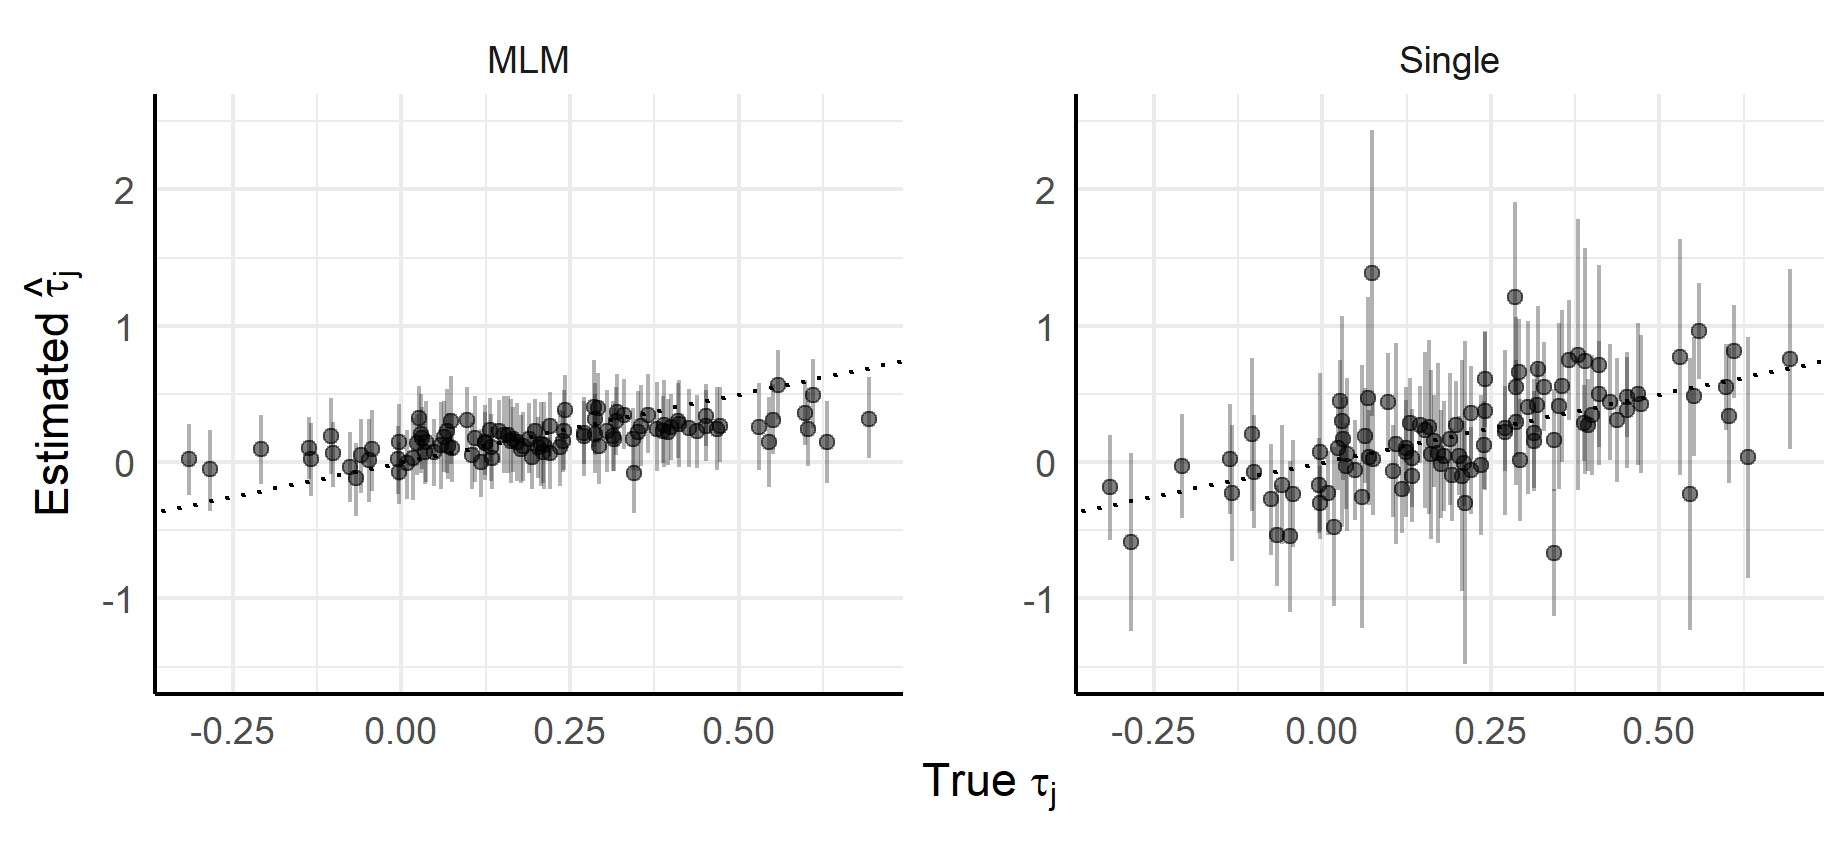
\includegraphics[width=\textwidth]{shrinkageplot}
	\caption{Power (at $\alpha = 0.1$) vs. true site ATE}
	\label{fig:example}
\end{figure}


\section{Simulation results}

Now we look at what happens upon repeated simulation.

\section{Case study}

\section{Conclusion}



\section{ORIGINAL WRITING}

Typically, researchers will power a multisite trial to ensure that a given design will achieve desired levels of power for the overall average treatment effect $\tau$ across all sites. 
In many applications, however, site stakeholders may be interested in estimating treatment effects $\tau_j$, $j = 1, \ldots, J$, at the individual sites as well.
To estimate site-level impacts, analysts typically use multilevel models (MLMs) to produce partially pooled estimates of the $\tau_j$.
For each site, these models ``borrow strength'' from the other sites, resulting in estimates $\hat{\tau}_j$ that are shrunken toward the estimated overall average treatment effect $\hat{\tau}$.
Standard Bayesian procedures may be used to construct credible intervals to conduct inference on these individual site-level effects.

The interpretation of these credible intervals requires some nuance, however.
There is an extensive literature concerning the construction of such intervals for individual site effects under shrinkage \citep{casella2012shrinkage}.
These intervals typically possess a so-called Empirical Bayes coverage property \citep{morris1983parametric}, i.e., they guarantee coverage for the collection of $\tau_j$ values \textit{on average} across all $J$ sites, not coverage for each individual $\tau_j$.
These guarantees may not be sufficient for stakeholders in multisite trials who would like to understand the effect of an experimental treatment at their particular site.
Overall, the question of inference for individual $\tau_j$ values in multilevel models remains fairly open \citep{armstrong2020robust}, with limited guidance about best practices.

\section{Objective}

In this paper, we provide guidance for analysts designing multisite trials with the knowledge that site stakeholders may be interested in individual site impact estimates.
We first demonstrate how naively applying standard power analysis methods to the multisite trial setting leads to unsatisfactory results, due to conflicts between Bayesian and Frequentist interpretations of coverage and power.
We then suggest a potential path forward.

% Similar power analyses have previously been conducted for the overall average treatment effect and cross-site variation in multisite trials \citep{raudenbush2000statistical}, but not for individual site-effect estimates, to the best of our knowledge.

% Two ideas to add:
% Idea 1: we're assuming exchangeability, so before the trial is run, everyone is the same to some extent?
% Idea 2: post-hoc power analyses are bad \href{https://statmodeling.stat.columbia.edu/2018/09/24/dont-calculate-post-hoc-power-using-observed-estimate-effect-size/}{says Gelman}

% We're doing a weird mix of pre- and post-trial stuff.
% In terms of coverage, things make sense.
% One idea: before we've run the analysis, what's the coverage of my intervals for sites with a true effect size of $\tau_j = 0.3$?
% Another idea: before we've run the analysis, what's the coverage of my intervals for sites with estimated $\hat{\tau}_j = 0.3$?

% In terms of power, things get weird.
% One idea: before we've run the analysis, what's the power of my procedure to detect effects at sites with $\tau_j = 0.3$?
% Another idea: before we've run the analysis, what's the power of my procedure to detect effects at sites with $\hat{\tau}_j = 0.3$?

% Is this second idea useful?
% Say I've run the trial and my observed $\hat{\tau}_j = 0.3$.
% The power analysis isn't useful at this point; I just have whatever interval I have, which says what it says.

% Something to note: power conditional on tau-hat depends strongly on the distribution of the $\tau_j$ values.
% Power conditional on $\tau_j$ depends less strongly on that, perhaps?

% The issue with post-hoc power analyses is...
% Plugging in $\hat{\tau}$ for $\tau$ is bad.
% Here, we're treating $\hat{\tau}_j$ and $\tau_j$ as completely different things, so it avoids those issues.


% Arc of the story: MLMs are bad if we're considering power at individual $\tau_j$ values.
% This is because individual CIs are by definition biased for individual $\tau_j$ values.
% This bias leads to weird coverage properties, and bad inferences.

% MLMs are good if we're considering power at individual $\hat{\tau}_j$ values.
% This is because shrinkage helps; based on the collection of sites, we can get information that an extreme $\hat{\tau}_j$ value is likely due to measurement error/noise, and not an extreme signal $\tau_j$.
% By pooling information, we are more likely to reject the null for any particular $\hat{\tau}_j$.

% TODO: study interval length

\section{Research Design}

We conduct a simulation study to explore power for individual site-level effects.
We repeatedly simulate data under a normal hierarchical model where we vary four data-generating parameters: the average size of each site $\bar{n}$, the number of sites $J$, the true overall average treatment effect $\tau$, and the true cross-site variation in site-level effects $\sigma^2_\tau$.
For each simulated dataset, we run four models: a normal Bayesian hierarchical model; a fixed-intercept, random-coefficients (FIRC) model \citep{bloom2017using}; a random-intercepts, random-coefficients (RIRC) model; and a separate t-test for each site. 

\section{Findings/Results}

% Updated framing idea:
% \begin{itemize}
%     \item ``MLMs improve EB power!'': Show power simulations for EB coverage/power
%     \begin{itemize}
%         \item TODO: presumably this works, need to check this
%     \end{itemize}
%     \item ``In a multisite trial, we might be tempted to power it to detect an effect at each individual site, in the same way we might power a study to detect an effect at a single site.
%         But really we should only consider EB power, since the usual Frequentist power criterion makes very little sense here'': Show Frequentist power analysis (conditional on $\tau_j$), and show that MLMs can become very bad.
%     \begin{itemize}
%         \item Note that this is worst when there is a lot of shrinkage.
%     \end{itemize}
%     \item ``This might look strange, but it's just because we're mixing frameworks'': Explain that this is because CIs from MLMs are Bayesian credible intervals, so in finite samples we shouldn't expect exact Frequentist coverage properties.
% \end{itemize}

% Open question: should we try to proceed from here?
% \begin{itemize}
%     \item It doesn't really make sense to discuss Frequentist power since Frequentist coverage of these intervals is wrong, by definition
%     \item It also doesn't really make sense to discuss Bayesian power since Bayesian notions of power usually integrate over the distribution of $\tau_j$, i.e., aren't ``for each individual site.''
%         \begin{itemize}
%             \item I.e., the intuition is that before we see anything, we know that our procedure will have good coverage because sites are exchangeable.
%             \item Once a true $\tau_j$ is drawn and conditioned on, however, all bets are off.
%         \end{itemize}
% \end{itemize}

% Ideally: we'd ``provide the thinking about how to discuss and calculate power for individual sites, as well as give a simulation to see how different approaches can break down.''
% Practically speaking, it's challenging to think about what this ``power for individual sites'' piece means.

% Robust EBCIs... EB confidence intervals that are robust to distribution of $\tau_j$ values!

% \newpage

In a traditional power analysis, the analyst posits an effect size $c$ and computes power (at level $\alpha$).
An analogous procedure for site-level effects in a multisite trial would be to fix a true site-level effect $c$ and compute power as the probability of rejecting the null when the true site-level effect is $c$.
Figure \ref{fig:power_plot} visualizes the results of a power simulation under this setup.
The power of a one-sided hypothesis test for a positive effect is plotted against the true site-level effect size $\tau_j$.
Ideally, the power curves would be less than $\alpha = 0.1$ for $\tau_j \leq 0$ to ensure test validity and high for $\tau_j > 0$ to maximize test power.
\begin{figure}[ht]
	\centering
	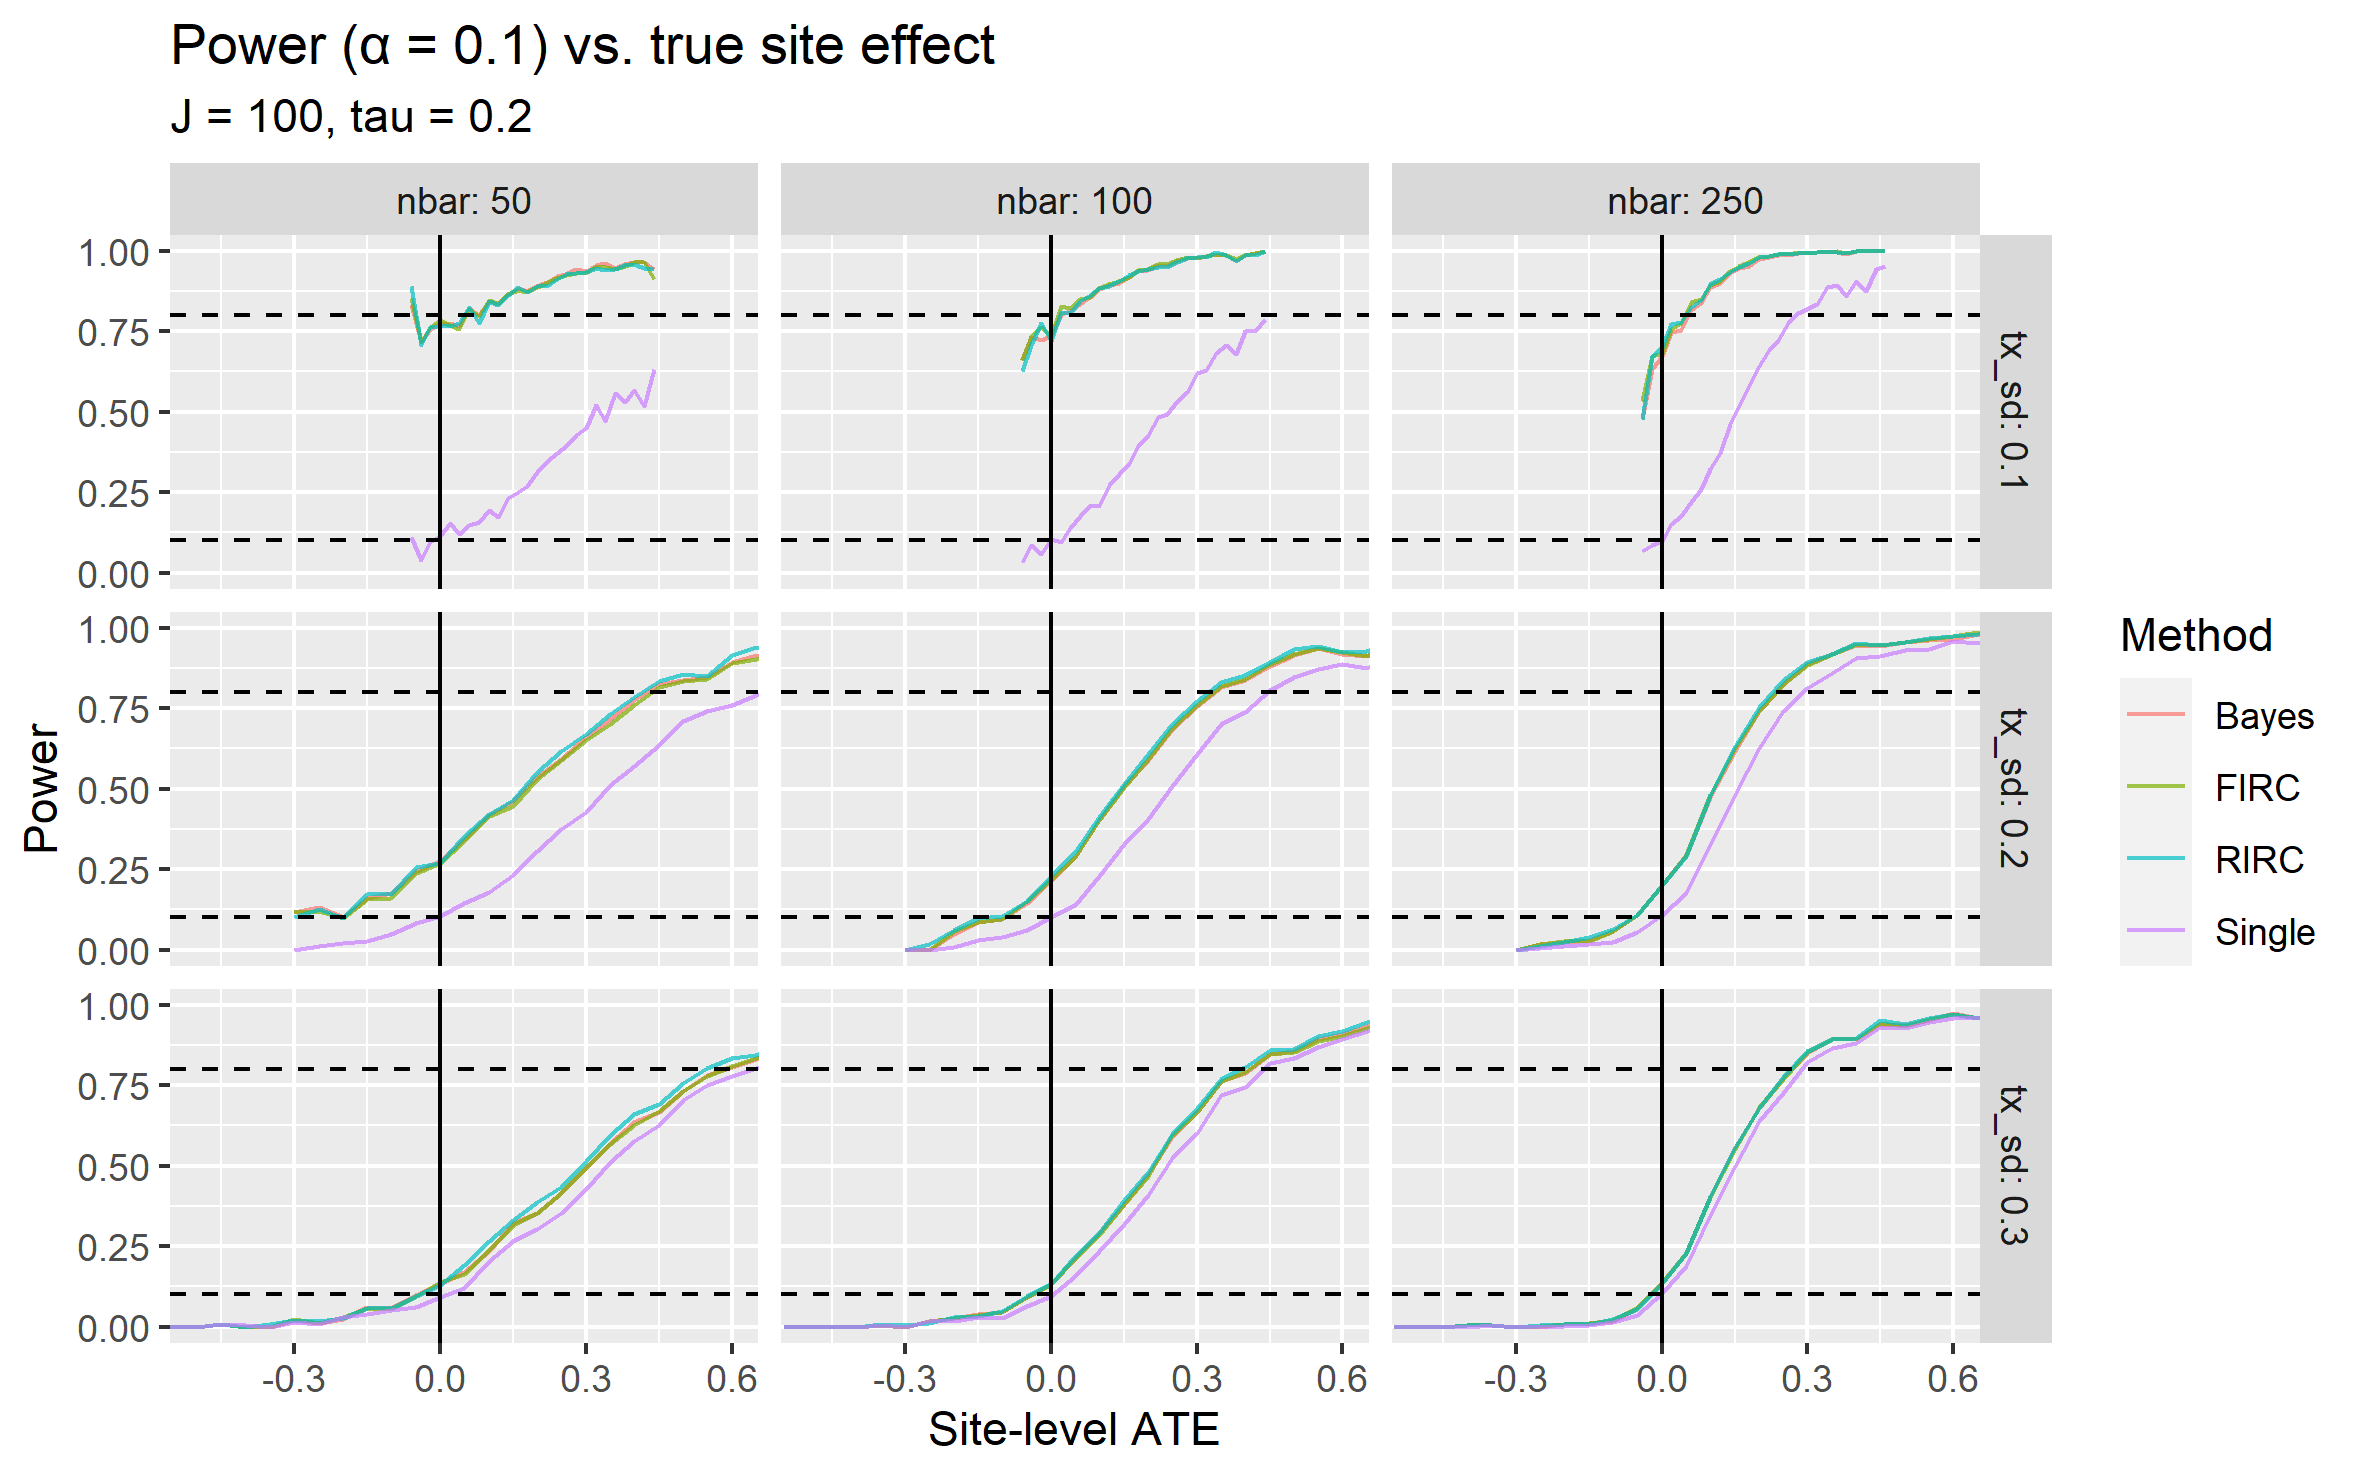
\includegraphics[width=\textwidth]{power_plot_J100}
	\caption{Power (at $\alpha = 0.1$) vs. true site ATE}
	\label{fig:power_plot}
\end{figure}

We see that while using MLMs improve power relative to estimating each site separately, these improvements often come at the cost of test validity.
This result holds for all of the MLMs in all settings, and is particularly extreme when cross-site variation is low ($\sigma_\tau = 0.1$), where the false positive rate for sites with negative $\tau_j$ values is nearly 80\%.

This behavior is expected for MLMs when power is computed at fixed values of $\tau_j$: MLMs naturally shrink estimates for sites with unusually small $\tau_j$ values toward the estimated overall mean, which is closer to $\tau = 0.2$.
The MLMs therefore estimate more positive effects for sites with negative $\tau_j$ values, resulting in many false rejections, particularly when the amount of cross-site impact variation is estimated to be small, causing shrinkage to be strong.
This naturally results in interval undercoverage (and falsely inflated power) for sites with true $\tau_j$ values far from the overall mean, as demonstrated in Figure \ref{fig:coverage_plot}.
\begin{figure}[ht]
	\centering
	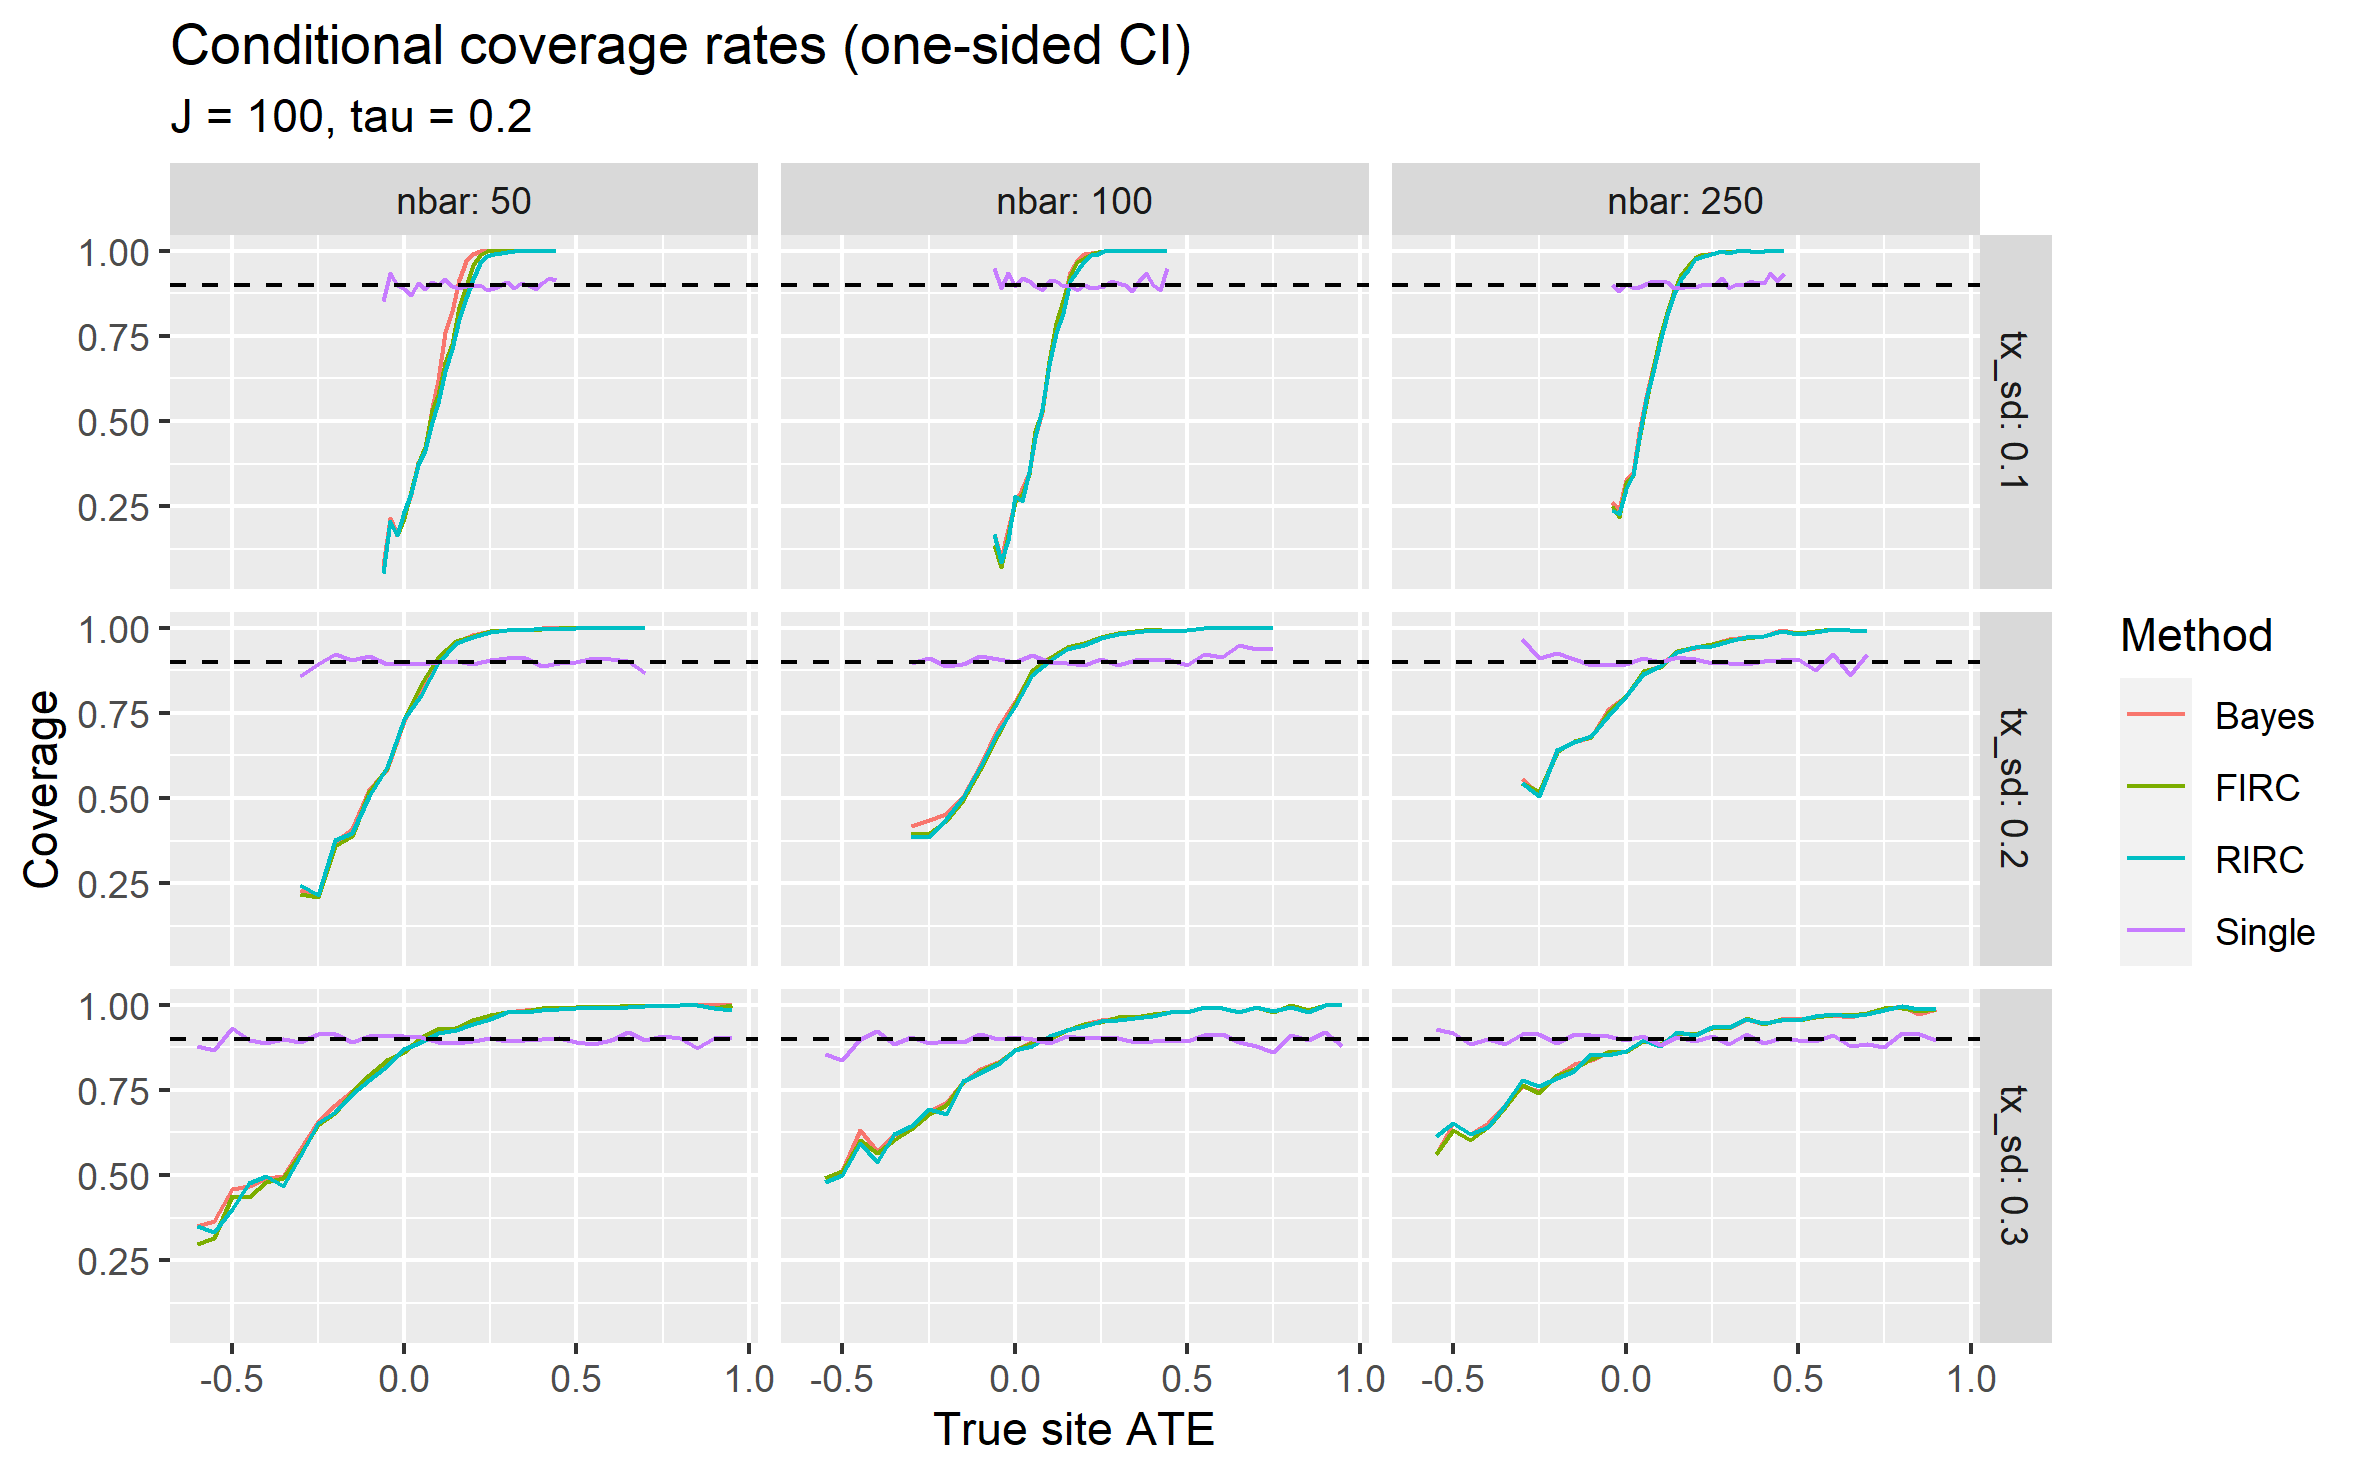
\includegraphics[width=\textwidth]{writeup/images/coverage_plot.png}
	\caption{Coverage (at $\alpha = 0.1$) vs. true site ATE}
	\label{fig:coverage_plot}
\end{figure}

In other words, MLMs have poor Frequentist coverage properties for fixed $\tau_j$ values, unlike running separate t-tests for each site.
Even when MLMs are well-specified (as they are in our simulations), their Bayesian credible intervals on $\hat{\tau}_j$ are designed to have proper Empirical Bayes coverage rates for $\tau_j$ \textit{on average}, across the prior distribution of true $\tau_j$ values, and not for any single, fixed $\tau_j$ value.
%\footnote{We note that in our simulations, Bayesian intervals indeed achieve roughly nominal Empirical Bayes coverage rates in most cases, except when shrinkage is very strong (e.g., low $\bar{n}$ and low $\sigma_\tau$).}
A naive power analysis that posits an effect size $\tau_j^*$ that the analyst would like to detect therefore leads to unsatisfactory results, since Bayesian notions of power and coverage are not defined conditional on fixed values of $\tau_j$.

Instead of naive Frequentist power analyses, we propose that analysts may conduct prospective interval-length analyses.
Using the simulation framework in this paper, an analyst can size a study to achieve a particular average interval width, across sites.
Figure \ref{fig:length_plot} demonstrates an example of this analysis.
\begin{figure}[ht]
	\centering
	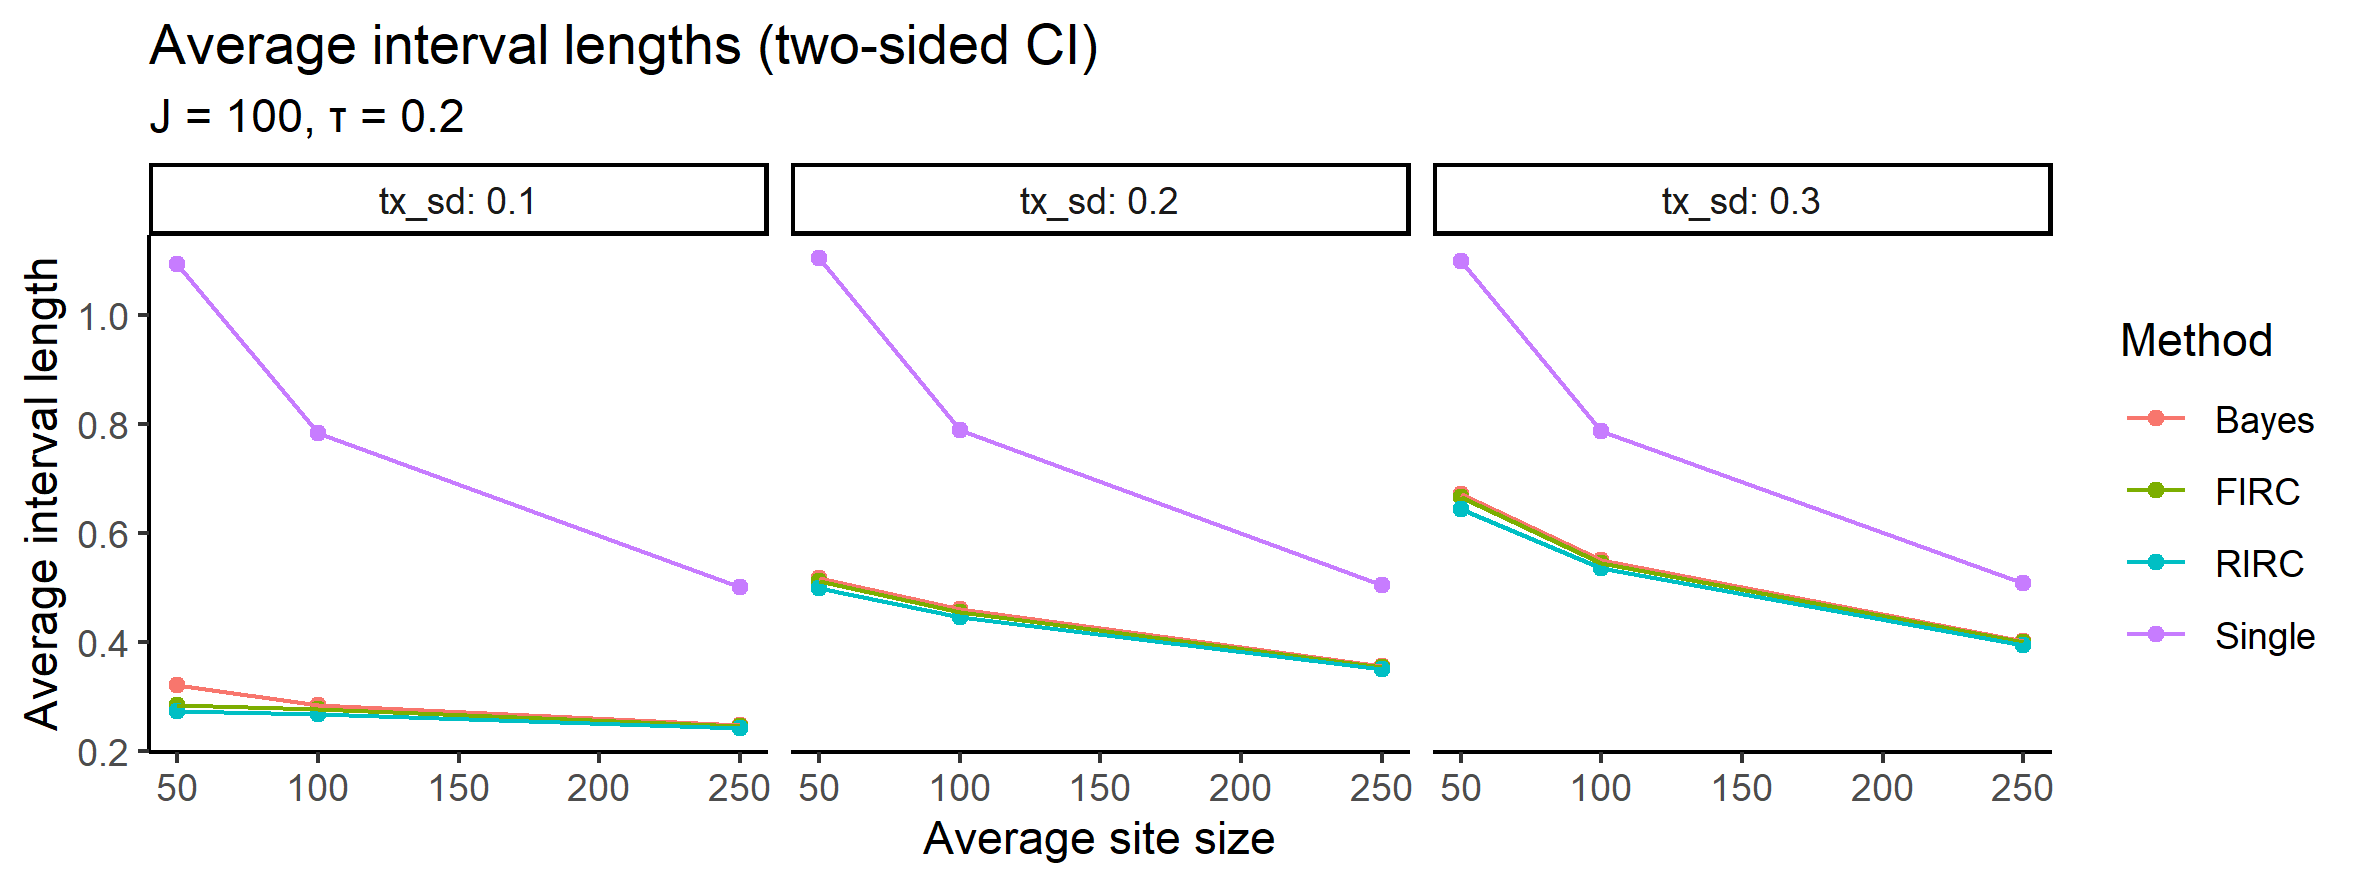
\includegraphics[width=\textwidth]{writeup/images/length_plot.png}
	\caption{Average two-sided credible interval length (at $\alpha = 0.1$)}
	\label{fig:length_plot}
\end{figure}
We see that using MLMs significantly decreases average interval length, particularly when $\sigma_\tau$ is small (i.e., shrinkage is high).
If, for example, an interval length of 0.4 is desirable for site stakeholders and treatment-effect variation is expected to be moderate ($\sigma_\tau$ = 0.2), an analyst may note that the 100 sites would have to reasonably large ($\bar{n} \approx 250$) in order to achieve the desired interval length on average.

% MLMs, however, have excellent coverage properties and power \textit{for fixed $\hat{\tau}_j$ values} when they are well-specified.
% Figure \ref{fig:power_plot_cond} replicates Figure \ref{fig:power_plot}, except now test powers (i.e., rejection rates) are computed for fixed $\hat{\tau}_j$ values rather than for fixed $\tau_j$ values.
% \begin{figure}[ht]
% 	\centering
% 	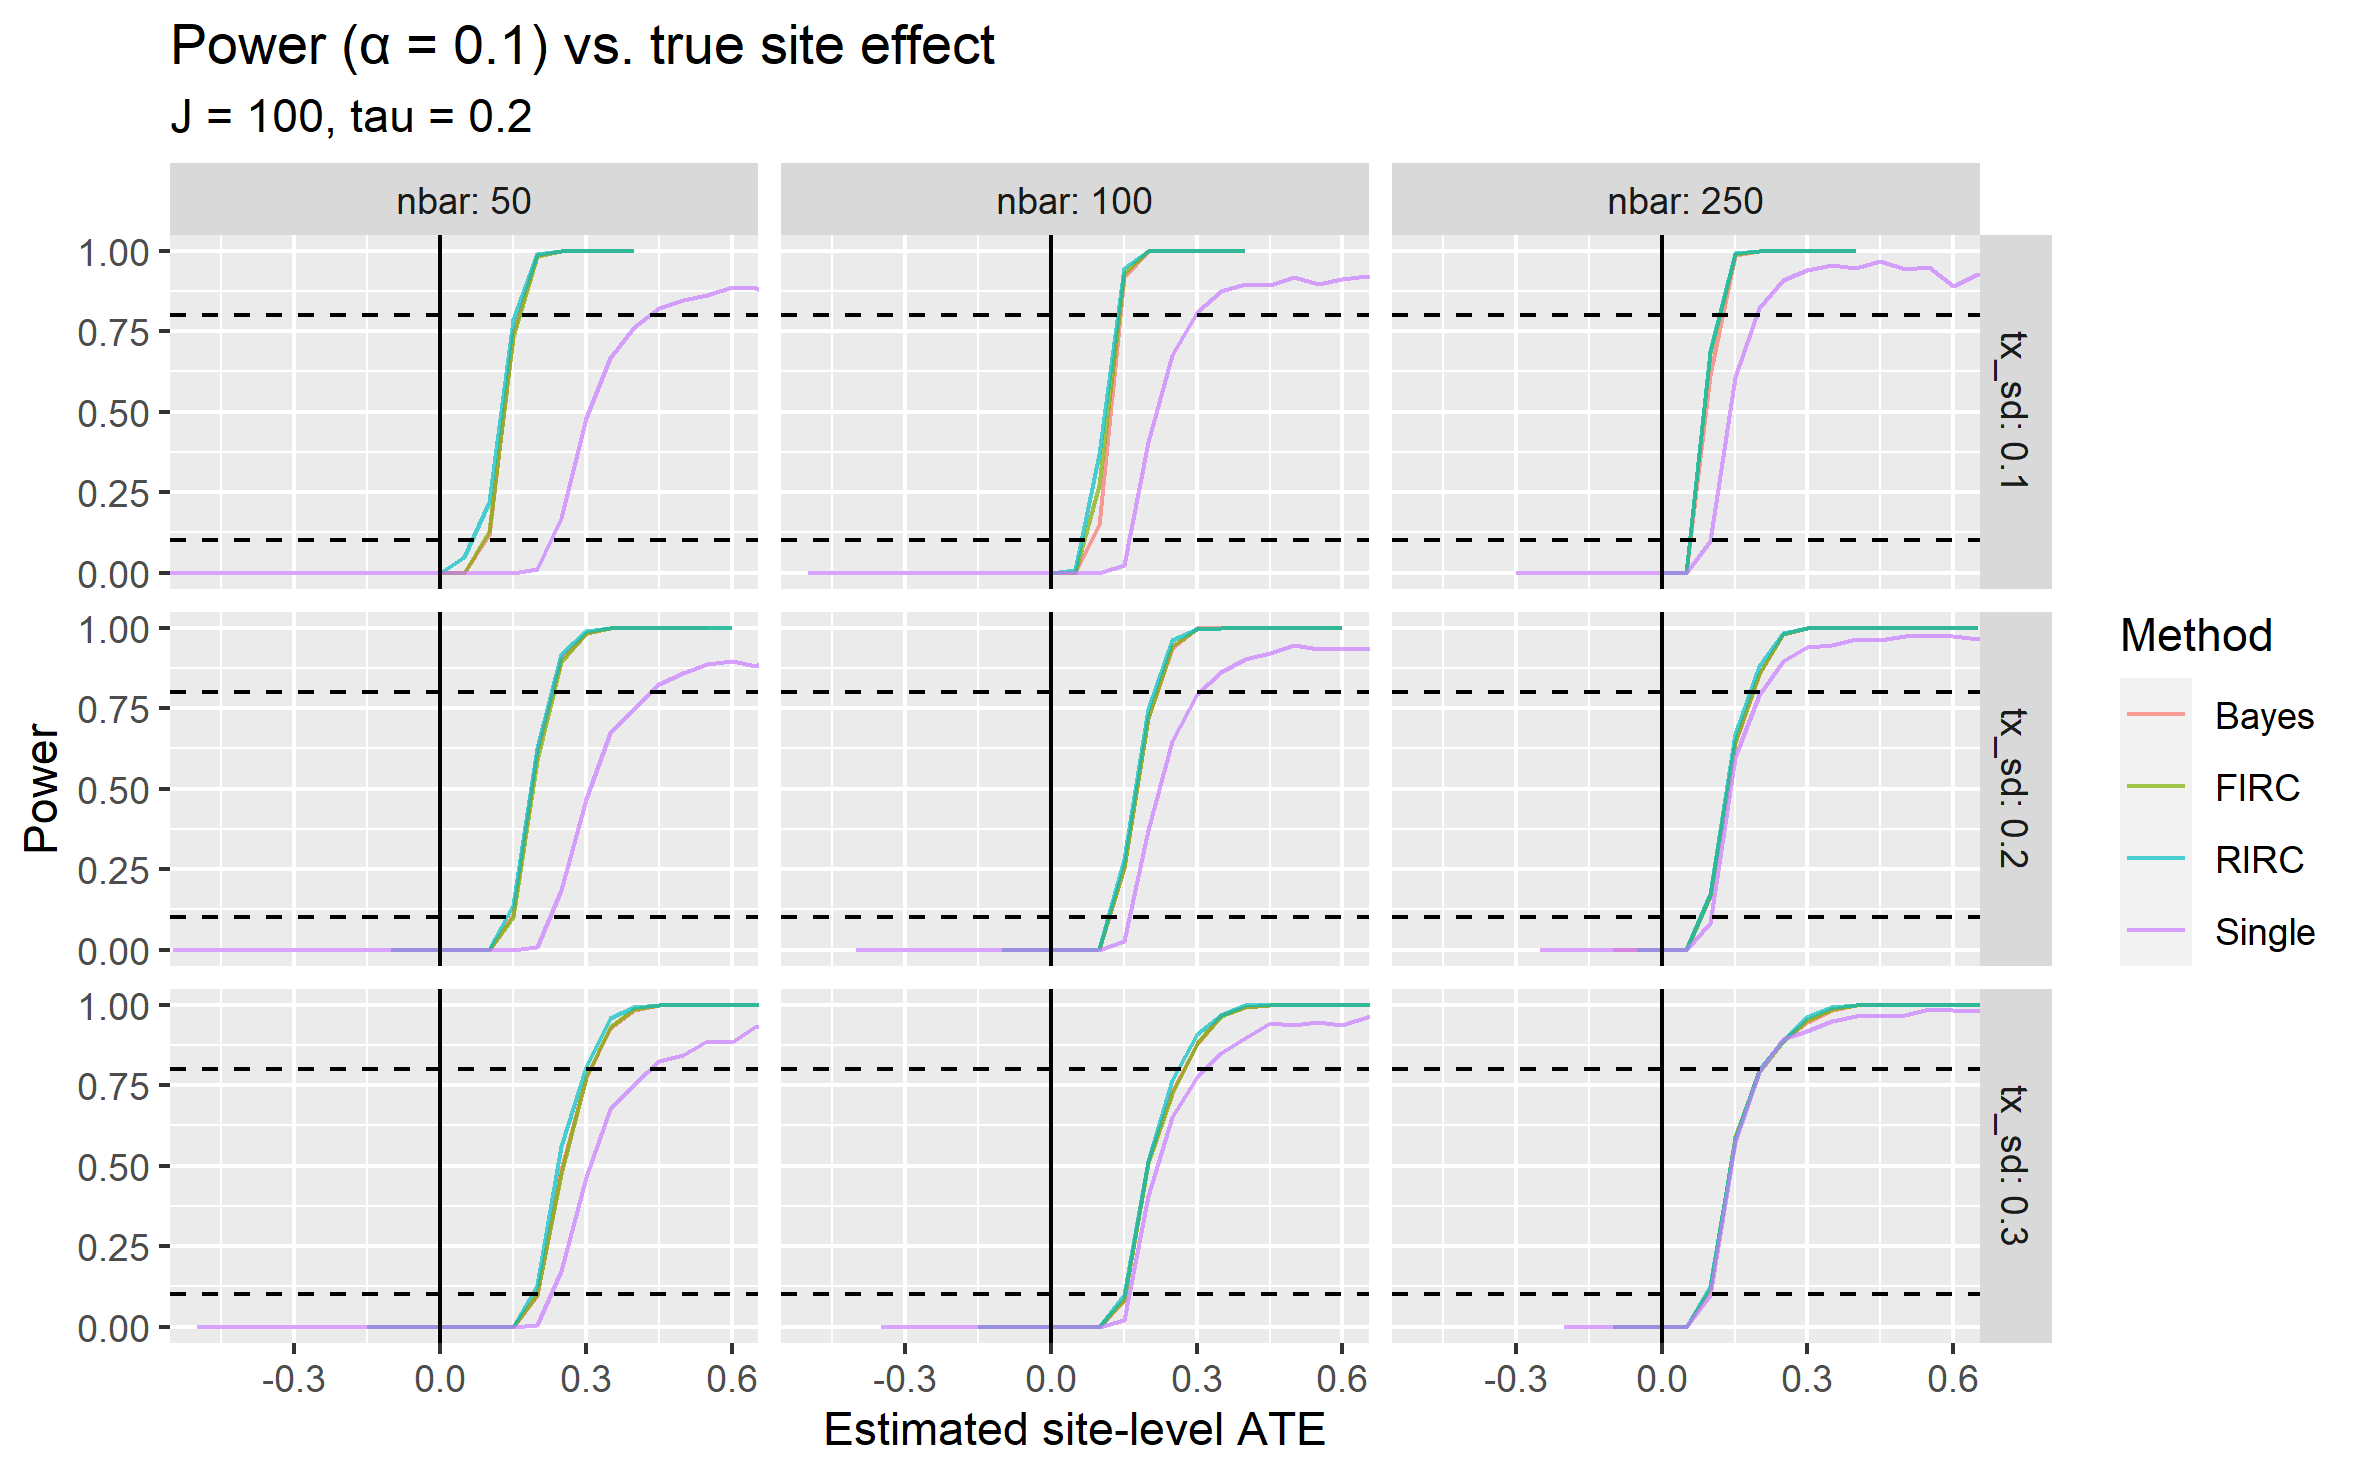
\includegraphics[width=\textwidth]{cond_power_1sided}
% 	\caption{Power (at $\alpha = 0.1$) vs. estimated site ATE}
% 	\label{fig:power_plot_cond}
% \end{figure}
% Under this setup, we see that the MLMs have significantly greater power than the individual t-tests.
% Figure \ref{fig:coverage_plot_cond} also shows that the coverage rates for the MLMs are generally correct.
% \begin{figure}[ht]
% 	\centering
% 	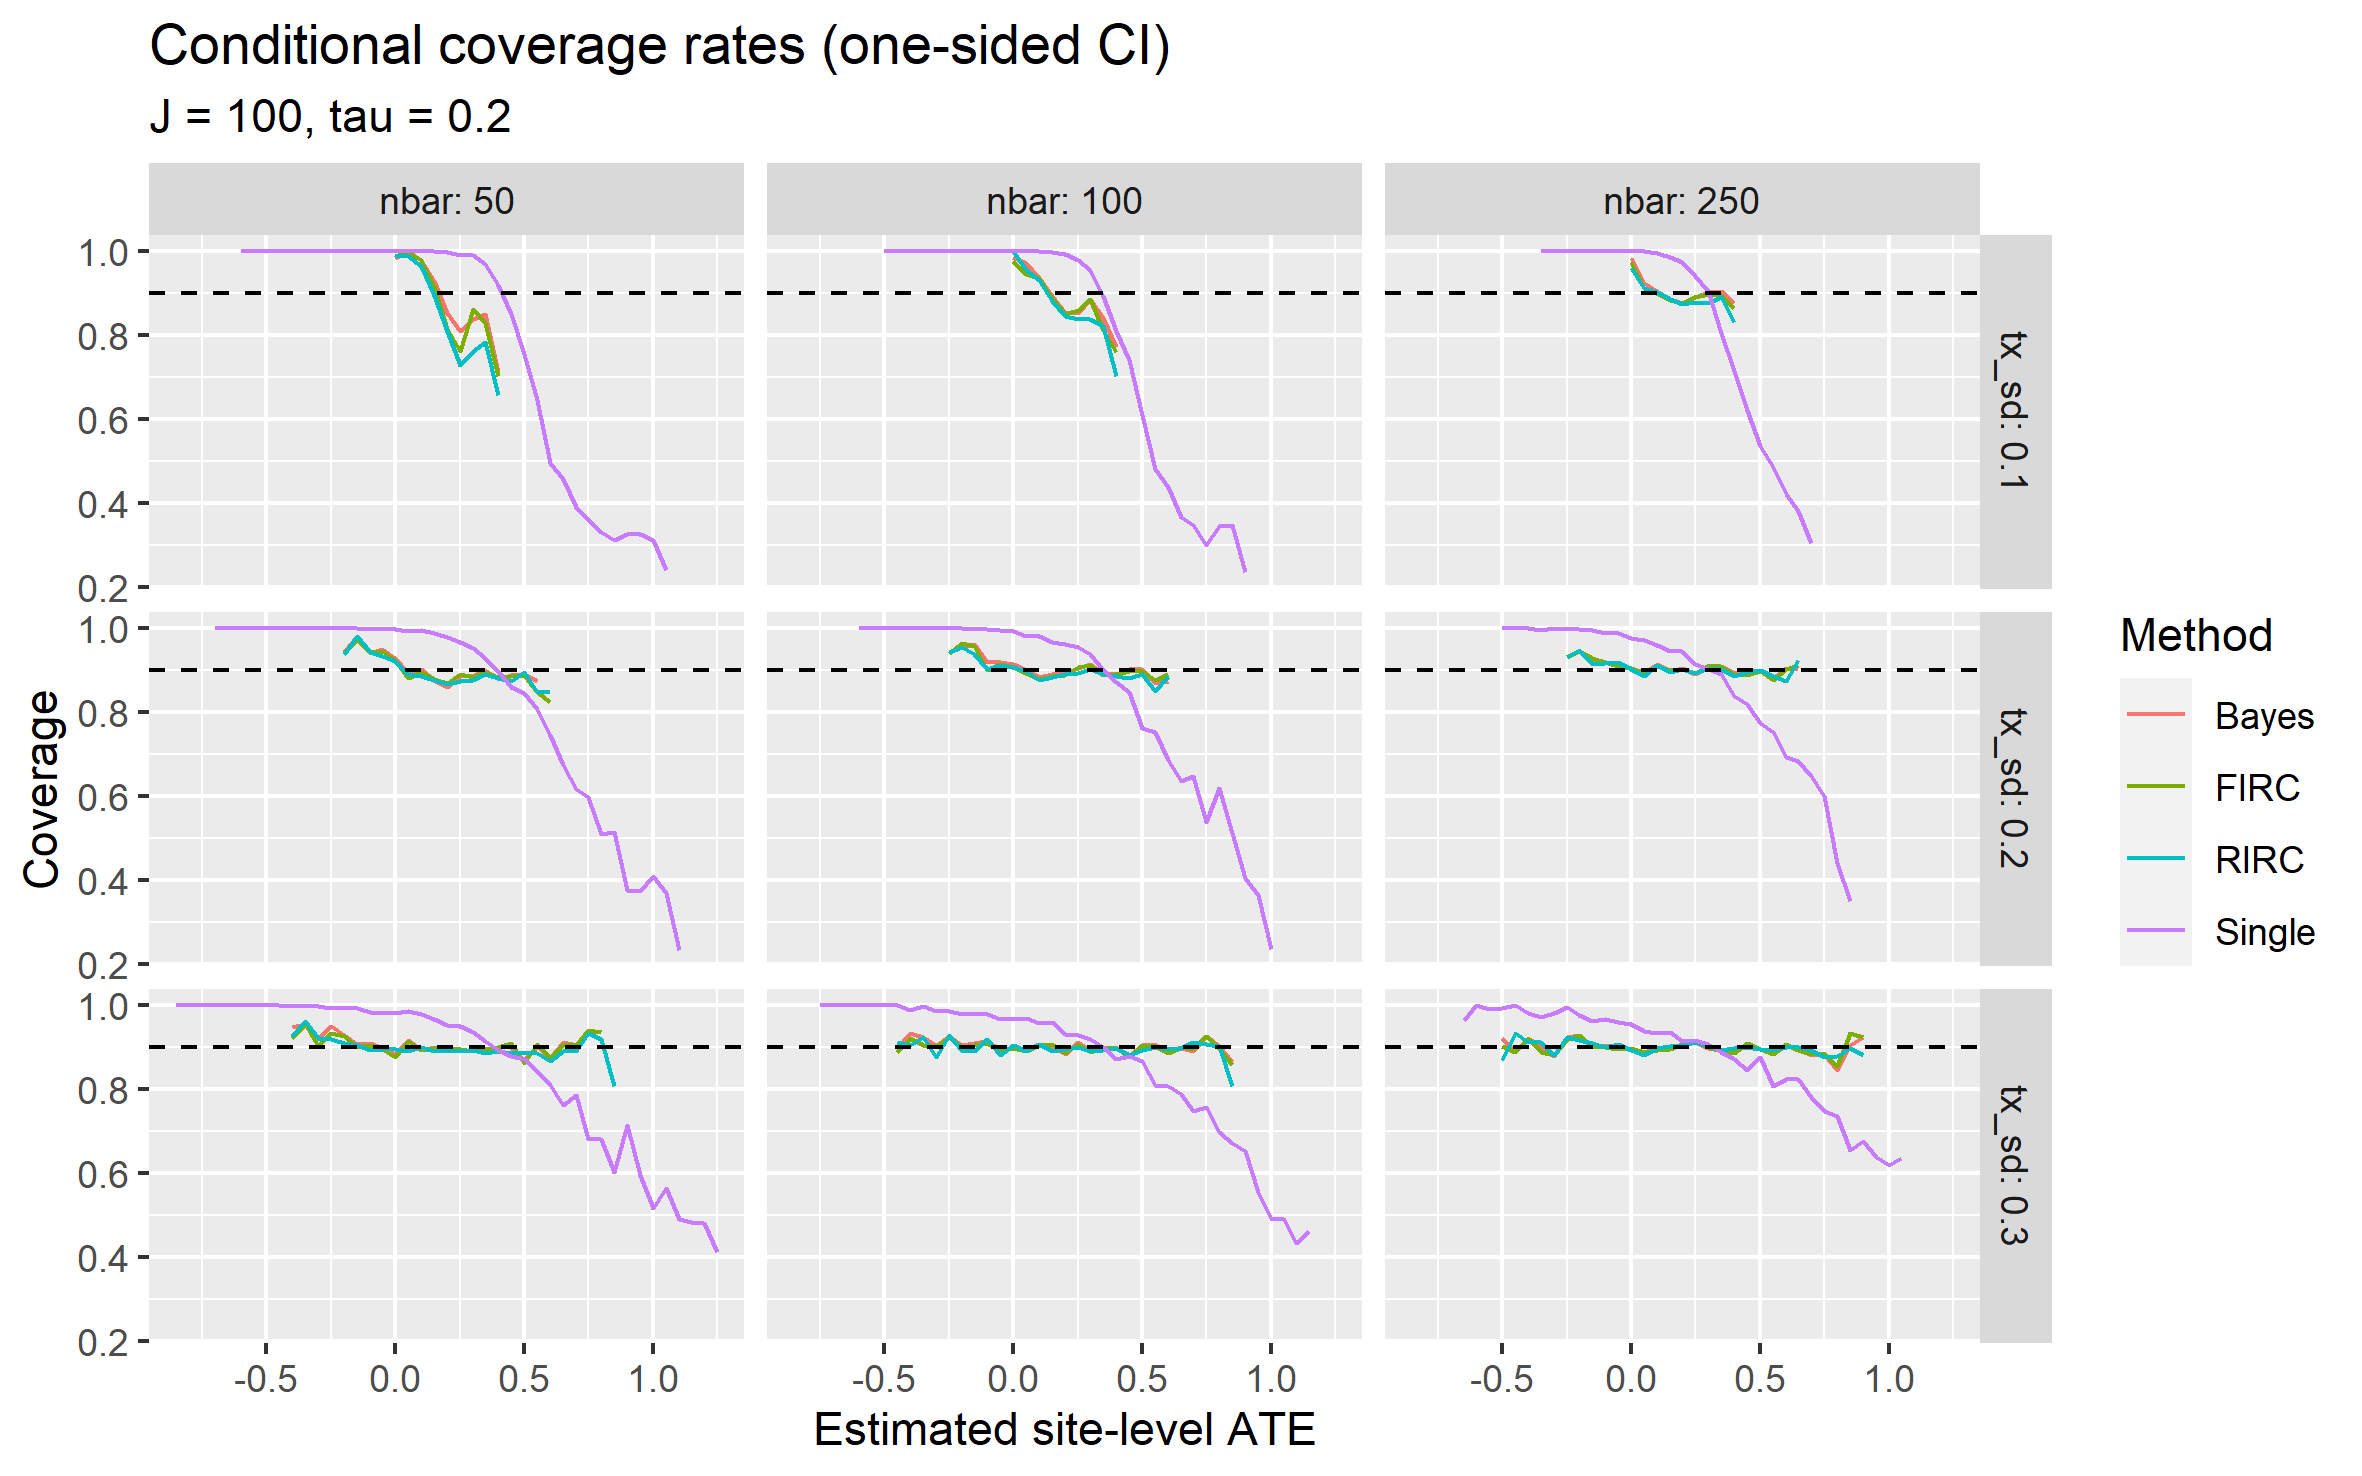
\includegraphics[width=\textwidth]{writeup/images/cond_coverage_1sided.png}
% 	\caption{Coverage (at $\alpha = 0.1$) vs. estimated site ATE}
% 	\label{fig:coverage_plot_cond}
% \end{figure}

% The results in Figures \ref{fig:power_plot_cond} and \ref{fig:coverage_plot_cond} are due to the MLMs appropriately shrinking extreme site-level effect estimates.
% Estimated site-level effects $\hat{\tau}_j$ may be extreme either because $\tau_j$ is extreme or because of random noise.
% MLMs use shrinkage to account for the fact that the majority of extreme $\hat{\tau}_j$ estimates are due to random noise rather than actual extreme signals; as a result, we see in our simulations that they produce intervals with better coverage rates than do individual site t-tests, particularly for large $\hat{\tau}_j$ values.
% Shrinkage also results in narrower intervals for sites with $\hat{\tau}_j$ close to the estimated overall average treatment effect, which improves power for those sites.


\section{Conclusions}

In many multisite trials, analysts may wish to power the trial to allow consistent detection of particular effect sizes at individual sites.
The credible intervals generated by MLMs, however, only guarantee average coverage rates across all sites, and not for sites with a fixed effect size $\tau_j$.
As a result, naive Frequentist power analyses for fixed $\tau_j$ values indicate that while MLMs have more power for detecting effects at individual sites than does separately testing each site, they are generally invalid.
Rather than performing naive Frequentist power analyses, analysts may consider running average-interval-length analyses.
Using the simulation framework in this paper, analysts may size a prospective study to achieve an average interval-length that stakeholders would be satisfied with for their individual site-level inferences.


\bibliography{refs.bib}
	
\end{document}